\documentclass[11pt]{article}
\usepackage{amsmath, amssymb, physics, mathtools, bm}
\usepackage{tikz, pgfplots}
\usetikzlibrary{calc, positioning, decorations.pathmorphing}
\pgfplotsset{compat=1.18}
\usepackage[margin=2.3cm]{geometry}
\usepackage{siunitx, booktabs, hyperref}
\newcommand{\D}{\mathrm{D}}
\newcommand{\de}{\mathrm{d}}
\newcommand{\pd}[2]{\frac{\partial #1}{\partial #2}}
\newcommand{\pdd}[2]{\frac{\partial^{2} #1}{\partial #2^{2}}}
\newcommand{\Lap}{\nabla^{2}}
\title{B2 Symmetry and Relativity, 2019 --- Model Solutions}
\author{}
\date{}
\begin{document}
\maketitle

%==================================================================
\section*{Question 1 --- Worldlines, constant-force motion, and causal structure}

\textbf{Problem.} Define proper time, 4-velocity $\bm U$, 4-acceleration $\bm A$ for $X^\mu(\tau)$; show $\bm U\cdot\bm A=0$. Constant 3-force $\bm f=(f_x,0,0)$ from rest: find $x(t),\dot x(t),\ddot x(t)$. Then draw causal diagrams of (0,0,0,0) in: (c) Minkowski + worldline of charged particle in $E_x$; (d) boosted axes; (e) compactified $x\equiv x+2\pi R$ with the same charged worldline; (f) compactified time $t\equiv t+2\pi T$.

\subsection*{(a) Proper time, 4-velocity, 4-acceleration}

Proper time is the invariant interval along a timelike worldline:
\[ c^2\de\tau^2 = -\de X\cdot\de X = c^2\de t^2 - \de\bm x^2. \]
4-velocity is the proper-time derivative of position:
\[ U^\mu = \frac{\de X^\mu}{\de\tau} = \gamma(c,\bm v). \]
4-acceleration is the proper-time derivative of 4-velocity:
\[ A^\mu = \frac{\de U^\mu}{\de\tau} = \gamma\frac{\de}{\de t}(\gamma c,\gamma\bm v). \]
Compute $U\cdot U$ with metric $(-,+,+,+)$:
\[ U\cdot U = -\gamma^2 c^2 + \gamma^2 v^2. \]
Factor $\gamma^2$:
\[ U\cdot U = \gamma^2(v^2 - c^2). \]
Use $\gamma^2 = 1/(1-v^2/c^2)$:
\[ U\cdot U = -c^2. \]
Differentiate with respect to $\tau$:
\[ \frac{\de}{\de\tau}(U\cdot U) = 2\,U\cdot A. \]
Set equal to zero since the right-hand side is constant:
\[ 2\,U\cdot A = 0. \]
Hence
\begin{equation}
\boxed{\bm U\cdot\bm A = 0.}
\end{equation}

\subsection*{(b) Constant 3-force from rest}

Newton-II in relativistic form, with $\bm p=\gamma m\bm v$:
\[ \frac{\de p_x}{\de t} = f_x. \]
Integrate with $p_x(0)=0$:
\[ p_x = f_x t. \]
Relate momentum to velocity via $p_x = \gamma m v_x$:
\[ \gamma m v_x = f_x t. \]
Use the identity $\gamma^2 = 1 + (p/mc)^2$:
\[ \gamma = \sqrt{1 + (f_x t/mc)^2}. \]
Divide $p_x = \gamma m v_x$ by $\gamma m$:
\[ v_x = \frac{f_x t/m}{\sqrt{1+(f_x t/mc)^2}}. \]
Define $a \equiv f_x/m$ so $\dot x$ becomes:
\[ \dot x = \frac{at}{\sqrt{1+(at/c)^2}}. \]
Integrate $\dot x$ with $x(0)=0$:
\[ x(t) = \int_0^t\frac{a t'\,\de t'}{\sqrt{1+(a t'/c)^2}}. \]
Substitute $w=at'/c$, $\de w=(a/c)\,\de t'$:
\[ x(t) = \frac{c^2}{a}\int_0^{at/c}\frac{w\,\de w}{\sqrt{1+w^2}}. \]
Use $\de(\sqrt{1+w^2}) = w\,\de w/\sqrt{1+w^2}$:
\[ x(t) = \frac{c^2}{a}\left[\sqrt{1+w^2}\right]_0^{at/c}. \]
Evaluate at the limits:
\[ x(t) = \frac{c^2}{a}\left[\sqrt{1+(at/c)^2}-1\right]. \]
Differentiate $\dot x = at/\sqrt{1+(at/c)^2}$ by the quotient rule:
\[ \ddot x = \frac{a\sqrt{1+(at/c)^2} - at\cdot\frac{a^2 t/c^2}{\sqrt{1+(at/c)^2}}}{1+(at/c)^2}. \]
Combine numerator over the common surd $\sqrt{1+(at/c)^2}$:
\[ \ddot x = \frac{a[1+(at/c)^2] - a^3 t^2/c^2}{[1+(at/c)^2]^{3/2}}. \]
Expand the bracket $a[1+(at/c)^2]$:
\[ \ddot x = \frac{a + a^3 t^2/c^2 - a^3 t^2/c^2}{[1+(at/c)^2]^{3/2}}. \]
Cancel the $a^3 t^2/c^2$ terms:
\[ \ddot x = \frac{a}{[1+(at/c)^2]^{3/2}}. \]
Hence
\begin{equation}
\boxed{x(t) = \frac{c^2}{a}\!\left[\sqrt{1+(at/c)^2}-1\right],\ \dot x = \frac{at}{\sqrt{1+(at/c)^2}},\ \ddot x = \frac{a}{[1+(at/c)^2]^{3/2}},\ a=f_x/m.}
\end{equation}
Limits: $at\ll c\Rightarrow x\to\tfrac12 a t^2$, $\dot x\to a t$; $at\gg c\Rightarrow\dot x\to c$, $\ddot x\to 0$.

\subsection*{(c) Minkowski causal structure with charged worldline}

Future light-cone of $O$: $|x|<ct,\ t>0$ (region I, can be affected by $O$). Past light-cone: $|x|<-ct,\ t<0$ (region II, can affect $O$). Elsewhere (spacelike, $|x|>c|t|$, region III) is causally disconnected.

Charged particle from rest in $(E_x,0,0)$: $f_x=qE_x$ constant, hyperbolic worldline from (b)
\[ x(t) = \frac{c^2}{a}\left[\sqrt{1+(at/c)^2}-1\right],\qquad a=qE_x/m. \]
Take $t\to+\infty$ so $\sqrt{1+(at/c)^2}\sim at/c$:
\[ x \to \frac{c^2}{a}\left(\frac{at}{c}-1\right) = ct - \frac{c^2}{a}. \]
The worldline asymptotes to the light-cone but never crosses it.

\begin{center}
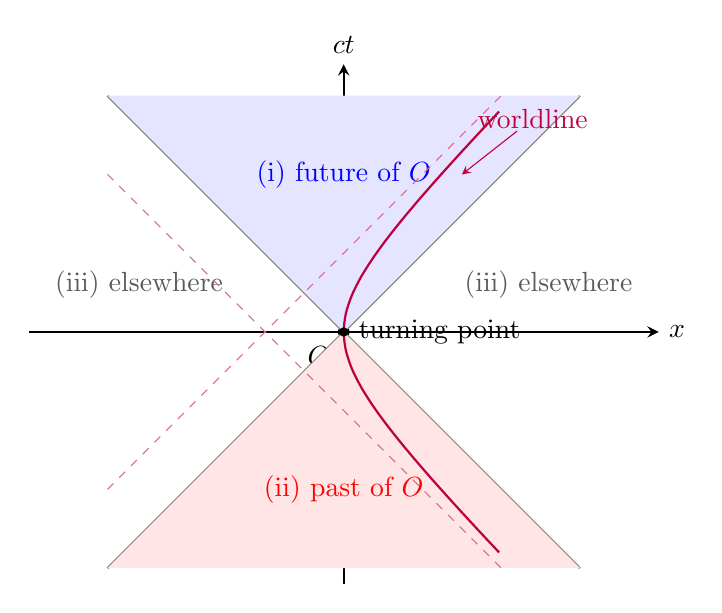
\begin{tikzpicture}[>=stealth, scale=1.0]
  % axes
  \draw[->, thick] (-4.0,0) -- (4.0,0) node[right] {$x$};
  \draw[->, thick] (0,-3.2) -- (0,3.4) node[above] {$ct$};
  \node[circle,fill,inner sep=1.5pt,label=below left:{$O$}] at (0,0) {};
  % light cones
  \draw[thick,gray] (-3.0,3.0) -- (3.0,-3.0);
  \draw[thick,gray] (-3.0,-3.0) -- (3.0,3.0);
  % Future cone shading
  \fill[blue!10] (0,0) -- (3.0,3.0) -- (-3.0,3.0) -- cycle;
  % Past cone shading
  \fill[red!10] (0,0) -- (3.0,-3.0) -- (-3.0,-3.0) -- cycle;
  % Region labels
  \node[blue] at (0,2.0) {(i) future of $O$};
  \node[red] at (0,-2.0) {(ii) past of $O$};
  \node[gray!70!black] at (2.6,0.6) {(iii) elsewhere};
  \node[gray!70!black] at (-2.6,0.6) {(iii) elsewhere};
  % Hyperbolic worldline: x = sqrt(1+t^2)-1 (a=c=1 in plot units)
  \draw[domain=-2.8:2.8,smooth,variable=\t,thick,purple]
    plot ({sqrt(1+\t*\t)-1},{\t});
  % asymptotes (dashed)
  \draw[dashed,purple!60] (-3.0,-2.0) -- (2.0,3.0);
  \draw[dashed,purple!60] (-3.0,2.0) -- (2.0,-3.0);
  % marker on worldline at t=0
  \node[circle,fill,inner sep=1.2pt,label=right:{turning point}] at (0,0) {};
  \node[purple] at (2.4,2.7) {worldline};
  \draw[purple,->,thin] (2.2,2.55) -- (1.5,2.0);
\end{tikzpicture}
\end{center}

\subsection*{(d) Boosted coordinates}

A standard boost rotates both axes inward by the same hyperbolic angle $\phi$, $\tanh\phi=v/c$: $t'$-axis tilts toward the future light-cone, $x'$-axis tilts symmetrically toward it from the right. The light-cone itself, and therefore the three causal regions (i)/(ii)/(iii), are unchanged.

\begin{center}
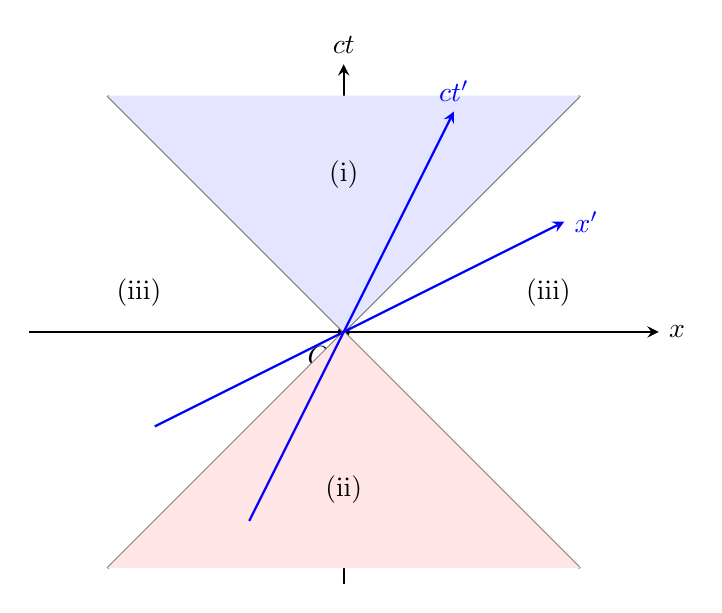
\begin{tikzpicture}[>=stealth, scale=1.0]
  \draw[->, thick] (-4.0,0) -- (4.0,0) node[right] {$x$};
  \draw[->, thick] (0,-3.2) -- (0,3.4) node[above] {$ct$};
  \node[circle,fill,inner sep=1.5pt,label=below left:{$O$}] at (0,0) {};
  % light cones
  \draw[thick,gray] (-3.0,3.0) -- (3.0,-3.0);
  \draw[thick,gray] (-3.0,-3.0) -- (3.0,3.0);
  \fill[blue!10] (0,0) -- (3.0,3.0) -- (-3.0,3.0) -- cycle;
  \fill[red!10] (0,0) -- (3.0,-3.0) -- (-3.0,-3.0) -- cycle;
  % boosted axes (phi = atan(0.5))
  \draw[->, thick, blue] (-2.4,-1.2) -- (2.8,1.4) node[right] {$x'$};
  \draw[->, thick, blue] (-1.2,-2.4) -- (1.4,2.8) node[above] {$ct'$};
  \node[blue] at (2.6,1.05) {};
  \node at (0,2.0) {(i)};
  \node at (0,-2.0) {(ii)};
  \node at (2.6,0.5) {(iii)};
  \node at (-2.6,0.5) {(iii)};
\end{tikzpicture}
\end{center}

The light-cone is invariant: causal regions are independent of frame.

\subsection*{(e) Compact spatial dimension $x\equiv x+2\pi R$}

In the universal cover the light-cone is the same, but the identification $x\sim x+2\pi R$ folds it back. Light from $O$ reaches every point on the spatial circle by $t=\pi R/c$ (going both ways). For $t>\pi R/c$ \emph{every} spatial point lies inside the future cone; similarly the past cone covers all space for $t<-\pi R/c$. The ``elsewhere'' region is confined to the strip $|t|<\pi R/c$ excluding the local Minkowski cones.

\begin{center}
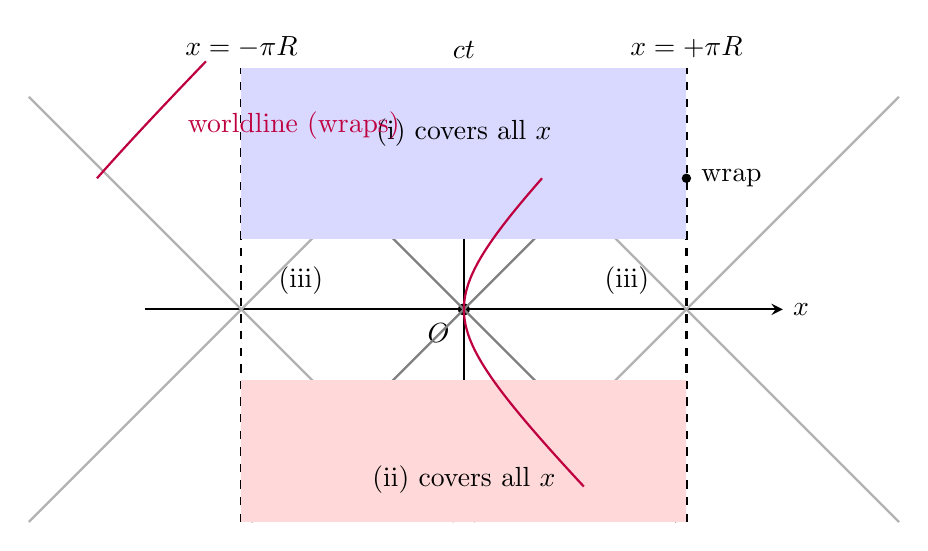
\begin{tikzpicture}[>=stealth, scale=0.9]
  % cylinder unfolded; show fundamental domain x in [-piR, piR]
  \draw[->, thick] (-4.5,0) -- (4.5,0) node[right] {$x$};
  \draw[->, thick] (0,-3.0) -- (0,3.4) node[above] {$ct$};
  \node[circle,fill,inner sep=1.5pt,label=below left:{$O$}] at (0,0) {};
  % identification lines
  \draw[dashed, thick] (-3.14,-3.0) -- (-3.14,3.4) node[above] {$x=-\pi R$};
  \draw[dashed, thick] ( 3.14,-3.0) -- ( 3.14,3.4) node[above] {$x=+\pi R$};
  % primary cone
  \draw[thick,gray] (-3.0,3.0) -- (3.0,-3.0);
  \draw[thick,gray] (-3.0,-3.0) -- (3.0,3.0);
  % image cones from x = +/- 2 pi R copies
  \draw[thick,gray!60] (-3.14-3.0,3.0) -- (-3.14+3.0,-3.0);
  \draw[thick,gray!60] (-3.14-3.0,-3.0) -- (-3.14+3.0,3.0);
  \draw[thick,gray!60] (3.14-3.0,3.0) -- (3.14+3.0,-3.0);
  \draw[thick,gray!60] (3.14-3.0,-3.0) -- (3.14+3.0,3.0);
  % fully covered future strip
  \fill[blue!15] (-3.14,1.0) rectangle (3.14,3.4);
  \fill[red!15]  (-3.14,-1.0) rectangle (3.14,-3.0);
  \node at (0,2.5) {(i) covers all $x$};
  \node at (0,-2.4) {(ii) covers all $x$};
  \node at (2.3,0.4) {(iii)};
  \node at (-2.3,0.4) {(iii)};
  % charged worldline (hyperbola, wrapping by identification when crossing x=piR)
  \draw[domain=-2.5:0,smooth,variable=\t,thick,purple]
    plot ({sqrt(1+\t*\t)-1},{\t});
  \draw[domain=0:1.85,smooth,variable=\t,thick,purple]
    plot ({sqrt(1+\t*\t)-1},{\t});
  \node[circle,fill,inner sep=1.2pt,label=right:{wrap}] at (3.14,1.85) {};
  \draw[domain=1.85:3.5,smooth,variable=\t,thick,purple]
    plot ({sqrt(1+\t*\t)-1-2*3.14},{\t});
  \node[purple] at (-2.4,2.6) {worldline (wraps)};
\end{tikzpicture}
\end{center}

The hyperbolic worldline of (c) wraps around the circle: each time $x$ reaches $+\pi R$ it reappears at $-\pi R$. The particle returns to its starting spatial point with $|\dot x|$ larger each time (the hyperbola $\dot x=at/\sqrt{1+(at/c)^2}$ is monotone), approaching $c$.

\medskip
\noindent\emph{Energy conservation.} A constant $\bm E$-field on a circle requires $\oint\bm E\cdot\de\bm\ell = 2\pi R E_x \neq 0$. By Faraday's law,
\[ \oint\bm E\cdot\de\bm\ell = -\dot\Phi_B, \]
so $\Phi_B$ through the circle decreases linearly with time at rate $-2\pi R E_x$. The work done on the particle each lap, $qE_x\cdot 2\pi R$, is supplied by the falling magnetic flux. Energy is conserved between particle and field; the assumption of a \emph{static, source-free} constant $\bm E$ is incompatible with the compactified topology, and a consistent solution requires the dynamical field source.

\subsection*{(f) Compact temporal dimension $t\equiv t+2\pi T$}

Closed timelike curves exist: every event lies on a closed loop $t\to t+2\pi T$ with $\bm x$ fixed. Hence \emph{every} event is to the future and to the past of $O$ simultaneously, so regions (i) and (ii) coincide and cover the whole spacetime; region (iii) is empty.
\begin{equation}
\boxed{(\text{i})=(\text{ii})=\text{all events},\qquad (\text{iii})=\varnothing.}
\end{equation}
This is inconsistent with causality: the grandfather paradox renders any local field theory ill-posed (no notion of initial data on a Cauchy surface, no global time-ordering). Compact time is therefore physically pathological.

%==================================================================
\section*{Question 2 --- Aberration, transverse Doppler, and resonant absorption by a moving cloud}

\textbf{Problem.} (a) Rod of length $L$ along $x'$ moves with $u\hat{\bm y}'$ in $S'$; $S'$ boosted by $v\hat{\bm x}$ relative to $S$. Find rod-angle in $S$. (b) Source at origin emits at $f_0$; observer with velocity $(0,v,0)$ passes through $(L,0,0)$ at $t=0$: derive $f(t)$ at observer, plot. (c) Replace observer by an unexcited atomic cloud (line $f$, lifetime $\tau$); plot amplitude and frequency at the source vs $t$ for several $v$, including the role of $f_0/f$ and intrinsic linewidth.

\subsection*{(a) Apparent angle of the moving rod}

Take the rod endpoints simultaneously in $S$ at time $t$, separated by $\Delta x$, $\Delta y$ in $S$. By length contraction along the boost direction:
\[ \Delta x = L/\gamma. \]
Apply the inverse Lorentz transform for time, $t' = \gamma(t - vx/c^2)$, at fixed $t$:
\[ \Delta t' = -\gamma v\,\Delta x/c^2. \]
Substitute $\Delta x = L/\gamma$:
\[ \Delta t' = -vL/c^2. \]
In $S'$ both endpoints move with $u\hat{\bm y}'$, so in this $\Delta t'$ the rightward endpoint shifts by $u\Delta t'$ in $y'$. Use $\Delta y = \Delta y'$ (no boost in $y$):
\[ \Delta y = u\,\Delta t' = -\frac{vuL}{c^2}. \]
Form the rod-vector $(\Delta x,\Delta y) = (L/\gamma,\,-vuL/c^2)$ and compute the angle:
\[ \tan\alpha = \frac{\Delta y}{\Delta x} = -\frac{vuL/c^2}{L/\gamma}. \]
Simplify the ratio:
\[ \tan\alpha = -\frac{\gamma v u}{c^2}. \]
Hence
\begin{equation}
\boxed{\tan\alpha = -\frac{\gamma v u}{c^2}.}
\end{equation}

\subsection*{(b) Doppler shift along the observer's path}

Observer position in $S$ at time $t$: $(L,vt,0)$. Photon emitted from the origin reaches it along
\[ \hat{\bm n}(t) = \frac{(L,vt,0)}{\sqrt{L^2+v^2t^2}}. \]
Define $\theta$ as the angle between $\hat{\bm n}$ and the observer velocity $v\hat{\bm y}$:
\[ \cos\theta = \hat{\bm n}\cdot\hat{\bm y} = \frac{vt}{\sqrt{L^2+v^2 t^2}}. \]
Photon 4-momentum: $P^\mu = (hf_0/c)(1,\hat{\bm n})$; observer 4-velocity: $U^\mu_{\rm obs} = \gamma(c,0,v,0)$. Observed energy is $-P_\mu U^\mu_{\rm obs}$:
\[ hf_{\rm obs} = -P_\mu U^\mu_{\rm obs} = \gamma hf_0(1 - \bm v\cdot\hat{\bm n}/c). \]
Divide through by $h$:
\[ f_{\rm obs} = \gamma f_0\bigl(1 - v\cos\theta/c\bigr). \]
Substitute $\cos\theta = vt/\sqrt{L^2+v^2t^2}$:
\[ f_{\rm obs}(t) = \frac{f_0}{\sqrt{1-v^2/c^2}}\left(1 - \frac{v^2 t}{c\sqrt{L^2+v^2 t^2}}\right). \]
Combine the bracket over a common denominator:
\[ f_{\rm obs}(t) = \frac{f_0\,(c\sqrt{L^2+v^2 t^2} - v^2 t)}{c\sqrt{L^2+v^2 t^2}\,\sqrt{1-v^2/c^2}}. \]
Hence
\begin{equation}
\boxed{f_{\rm obs}(t) = \frac{f_0}{\sqrt{1-v^2/c^2}}\left(1 - \frac{v^2 t}{c\sqrt{L^2+v^2 t^2}}\right).}
\label{eq:Q2b-fobs}
\end{equation}
Take $t\to-\infty$ so $\cos\theta\to-1$:
\[ f_{\rm obs}\to \gamma f_0(1+v/c). \]
Simplify with $\gamma(1+v/c) = \sqrt{(1+v/c)/(1-v/c)}$:
\[ f_{\rm obs}(-\infty) = f_0\sqrt{\frac{1+v/c}{1-v/c}}. \]
Take $t\to+\infty$ so $\cos\theta\to+1$:
\[ f_{\rm obs}\to \gamma f_0(1-v/c). \]
Apply the same identity:
\[ f_{\rm obs}(+\infty) = f_0\sqrt{\frac{1-v/c}{1+v/c}}. \]
At $t=0$ (transverse passage in $S$), $\cos\theta=0$:
\[ f_{\rm obs}(0) = \gamma f_0. \]
The observer approaches from $-y$ (blueshift) and recedes toward $+y$ (redshift); $f_{\rm obs}$ decreases monotonically through the transverse value $\gamma f_0$ at $t=0$.

\begin{center}
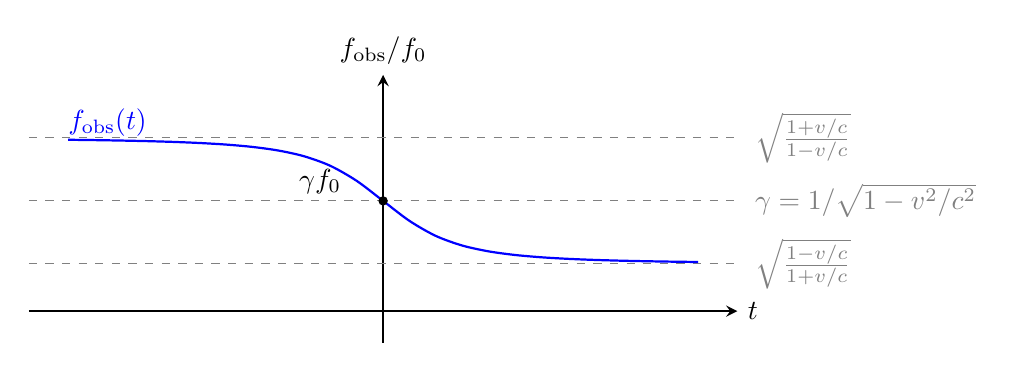
\begin{tikzpicture}[>=stealth, scale=1.0]
  \draw[->, thick] (-4.5,0) -- (4.5,0) node[right] {$t$};
  \draw[->, thick] (0,-0.4) -- (0,3.0) node[above] {$f_{\rm obs}/f_0$};
  % blue (approach, t<<0) and red (recede, t>>0) asymptotes
  \draw[dashed, gray] (-4.5,2.2) -- (4.5,2.2);
  \draw[dashed, gray] (-4.5,0.6) -- (4.5,0.6);
  \draw[dashed, gray] (-4.5,1.4) -- (4.5,1.4);
  \node[gray,right] at (4.6,2.2) {$\sqrt{\tfrac{1+v/c}{1-v/c}}$};
  \node[gray,right] at (4.6,0.6) {$\sqrt{\tfrac{1-v/c}{1+v/c}}$};
  \node[gray,right] at (4.6,1.4) {$\gamma=1/\sqrt{1-v^2/c^2}$};
  % monotone-decreasing S-curve through (0, gamma)
  \draw[domain=-4.0:4.0,smooth,variable=\t,thick,blue]
    plot ({\t},{1.4 - 0.8*\t/sqrt(1+\t*\t)});
  \node[circle,fill,inner sep=1.2pt] at (0,1.4) {};
  \node at (-0.8,1.65) {$\gamma f_0$};
  \node[blue] at (-3.5,2.4) {$f_{\rm obs}(t)$};
\end{tikzpicture}
\end{center}

\subsection*{(c) Resonant absorption by a moving atomic cloud and re-emission}

Atoms in cloud move with $\bm v=v\hat{\bm y}$. Source emits spherical waves at $f_0<f$. From \eqref{eq:Q2b-fobs}, the frequency seen by an atom is set by $\cos\theta(t)=vt/\sqrt{L^2+v^2 t^2}$:
\[ f_{\rm atom}(t) = \gamma f_0\bigl(1 - v\cos\theta(t)/c\bigr). \]
Resonance requires $|f_{\rm atom}-f|\lesssim\Gamma$, with the natural linewidth $\Gamma\sim 1/(2\pi\tau)$.

\textbf{Critical velocity $v_c$.} Maximum blueshift occurs at $\cos\theta=-1$ (atom approaching head-on, $t\to-\infty$):
\[ f_{\rm max}(v) = \gamma f_0(1+v/c). \]
Simplify using $\gamma(1+v/c) = \sqrt{(1+v/c)/(1-v/c)}$:
\[ f_{\rm max}(v) = f_0\sqrt{\frac{1+v/c}{1-v/c}}. \]
Resonance possible iff $f_{\rm max}(v)\geq f$. Setting $f_{\rm max}(v_c) = f$:
\[ \sqrt{\frac{1+v_c/c}{1-v_c/c}} = \frac{f}{f_0}. \]
Square both sides and solve for $v_c$:
\[ v_c = c\,\frac{(f/f_0)^2-1}{(f/f_0)^2+1}. \]

\medskip
\noindent\emph{Resonant angle.} Set $f_{\rm atom} = f$:
\[ \gamma f_0(1 - v\cos\theta_{\rm res}/c) = f. \]
Solve for $\cos\theta_{\rm res}$:
\[ \cos\theta_{\rm res} = \frac{c}{v}\left(1 - \frac{f}{\gamma f_0}\right). \]
At $v = v_c$, $f/(\gamma f_0) = 1+v/c$, giving $\cos\theta_{\rm res}=-1$ (resonance at head-on).
Resonance time $t_{\rm res}$ from $\cos\theta(t) = vt/\sqrt{L^2+v^2 t^2}$:
\[ t_{\rm res} = \frac{L\cos\theta_{\rm res}}{v\,\sin\theta_{\rm res}} = \frac{L\cos\theta_{\rm res}}{v\sqrt{1-\cos^2\theta_{\rm res}}}. \]
For $v$ just above $v_c$: $\cos\theta_{\rm res}\to-1$ so $t_{\rm res}\to-\infty$ (resonance with atom far away, approaching head-on). For $v\to c$: $\gamma\to\infty$ so $f/(\gamma f_0)\to 0$, giving $\cos\theta_{\rm res}\to 1$ and $t_{\rm res}\to+\infty$ (resonance after transverse passage, atom receding nearly head-on).

\medskip
\noindent\emph{Frequency of returning photon at source.} The excited atom (moving at $v\hat{\bm y}$ in $S$) re-emits at rest-frame frequency $f$; the photon travels back to the origin with direction $-\hat{\bm n}$ in $S$. Contract photon 4-momentum with atom 4-velocity, $-P_\mu U^\mu_{\rm atom} = hf$:
\[ hf = h f_{\rm src}\,\gamma(1+v\cos\theta/c). \]
Solve for the frequency at the source $f_{\rm src}$:
\[ f_{\rm src} = \frac{f}{\gamma(1+v\cos\theta/c)}. \]
Rewrite using $1/\gamma = \sqrt{1-v^2/c^2}$:
\[ f_{\rm src} = \frac{f\sqrt{1-v^2/c^2}}{1+v\cos\theta/c}. \]
At the resonance instant use $f/\gamma = f_0(1-v\cos\theta_{\rm res}/c)$:
\[ f_{\rm src}^{\rm res} = f_0\,\frac{1-v\cos\theta_{\rm res}/c}{1+v\cos\theta_{\rm res}/c}. \]

\medskip
\noindent\emph{Line width and decay.} The transition has finite linewidth $\Gamma\sim 1/(2\pi\tau)$, so resonance is met over a window $\Delta t$ set by $|\de f_{\rm atom}/\de t|^{-1}\Gamma$. After absorption, the cloud re-emits exponentially with timescale $\tau$, smearing the return echo by $e^{-(t-t_{\rm res})/\tau}$ for $t>t_{\rm res}$.

\medskip
\noindent\emph{Three regimes.}

\textbf{(i) $v\ll v_c$:} $f_{\rm max}<f$, no resonance. Absorption only through line wings: amplitude suppression $\propto\Gamma^2/(f-f_{\rm atom})^2$, exponentially small. Re-emitted signal at source negligible.

\textbf{(ii) $v\approx v_c$:} resonance only at $\cos\theta\to -1$, i.e.\ $t_{\rm res}\to-\infty$ (atom far away approaching head-on). Absorption window is broad and asymmetric (vanishing $|\de f_{\rm atom}/\de t|$ at extremes).

\textbf{(iii) $v_c < v < c$:} a single resonance angle $\cos\theta_{\rm res}\in(-1,1)$ gives a sharp absorption notch at $t_{\rm res}$ in the through-going signal, plus a re-emission echo at the source at frequency $f_{\rm src}^{\rm res}$, decaying over $\tau$.

\textbf{(iv) $v\to c$:} $\cos\theta_{\rm res}\to 1$, $t_{\rm res}\to+\infty$ (resonance occurs late, when the atom is far ahead and receding). Echo arrives at very late time, frequency-shifted strongly by the back-Doppler factor.

\medskip
\noindent\emph{Effect of $f_0/f$.} As $f_0/f\to 1$, $v_c\to 0$ (resonance for arbitrarily small $v$); as $f_0/f\to 0$ (very mismatched), $v_c\to c$ (only ultra-relativistic clouds resonate).

\medskip
\noindent\emph{Schematic plots ($v$ increasing left-to-right). Top: amplitude $A(t)$; bottom: frequency $f_{\rm src}(t)$ of returning radiation.}

\begin{center}
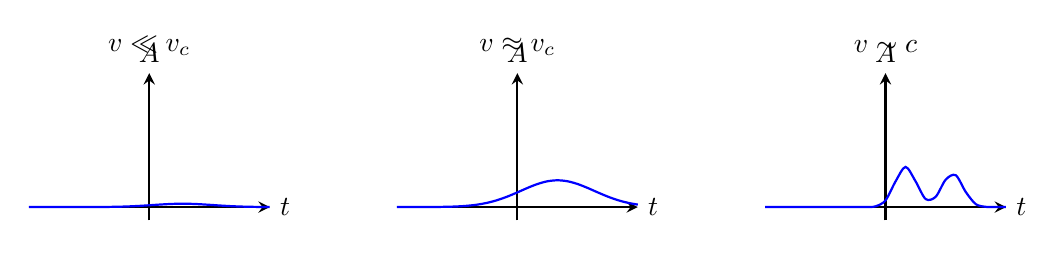
\begin{tikzpicture}[>=stealth, scale=0.85]
  % three panels: v << vc, v = vc, v >> vc
  \foreach \xc/\lab in {0/{$v\ll v_c$}, 5.5/{$v\approx v_c$}, 11.0/{$v\sim c$}} {
    \draw[->, thick] (\xc-1.8,0) -- (\xc+1.8,0) node[right] {$t$};
    \draw[->, thick] (\xc,-0.2) -- (\xc,2.0) node[above] {$A$};
    \node at (\xc,2.4) {\lab};
  }
  % v << vc: tiny bump
  \draw[domain=-1.8:1.8,smooth,variable=\t,thick,blue]
    plot ({\t},{0.05*exp(-(\t-0.5)*(\t-0.5)/0.4)});
  % v ~ vc: broader, asymmetric
  \draw[domain=-1.8:1.8,smooth,variable=\t,thick,blue]
    plot ({5.5+\t},{0.4*exp(-(\t-0.6)*(\t-0.6)/0.6)});
  % v >> vc: two dips/peaks
  \draw[domain=-1.8:1.8,smooth,variable=\t,thick,blue]
    plot ({11+\t},{0.6*exp(-(\t-0.3)*(\t-0.3)/0.05)+0.5*exp(-(\t-1.0)*(\t-1.0)/0.05)});
\end{tikzpicture}
\end{center}

\begin{center}
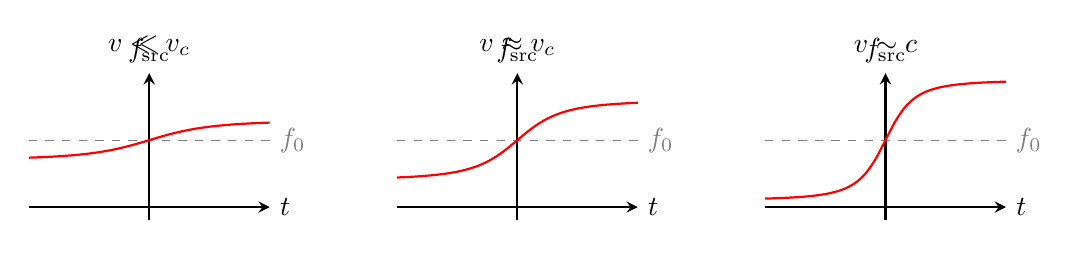
\begin{tikzpicture}[>=stealth, scale=0.85]
  \foreach \xc/\lab in {0/{$v\ll v_c$}, 5.5/{$v\approx v_c$}, 11.0/{$v\sim c$}} {
    \draw[->, thick] (\xc-1.8,0) -- (\xc+1.8,0) node[right] {$t$};
    \draw[->, thick] (\xc,-0.2) -- (\xc,2.0) node[above] {$f_{\rm src}$};
    \draw[dashed,gray] (\xc-1.8,1.0) -- (\xc+1.8,1.0);
    \node[gray,right] at (\xc+1.8,1.0) {$f_0$};
    \node at (\xc,2.4) {\lab};
  }
  % Plot frequency curves: monotone S-curves with small bumps where resonance occurs
  \draw[domain=-1.8:1.8,smooth,variable=\t,thick,red]
    plot ({\t},{1.0+0.3*\t/sqrt(1+\t*\t)});
  \draw[domain=-1.8:1.8,smooth,variable=\t,thick,red]
    plot ({5.5+\t},{1.0+0.6*\t/sqrt(0.5+\t*\t)});
  \draw[domain=-1.8:1.8,smooth,variable=\t,thick,red]
    plot ({11+\t},{1.0+0.9*\t/sqrt(0.2+\t*\t)});
\end{tikzpicture}
\end{center}

Key features: (1) carrier frequency at the source follows the relativistic Doppler curve of \eqref{eq:Q2b-fobs} (now interpreted as the source-to-atom-to-source two-step); (2) sharp resonant absorption notch whenever $f_{\rm obs}(t)=f$, of width $\sim\Gamma$; (3) re-emission echo after the absorption notch, decaying with $\tau$, frequency-shifted by the back-Doppler factor; (4) for $v<v_c$, no notches, only line-wing absorption.

%==================================================================
\section*{Question 3 --- 4-vectors, the EM tensor, and field invariants}

\textbf{Problem.} (a) Distinguish ``invariant'' vs ``conserved''; how do 4-vectors and tensors transform under Lorentz transformations? (b) Show: if $Y^\mu$ has a component zero in all frames, then $Y^\mu=0$; physical consequence; same for tensors? (c) Form of $A_\mu$ and $F_{\mu\nu}$; explicit $F_{\mu\nu}$ in terms of $\bm E,\bm B$; $\bm E,\bm B$ Lorentz transformations. (d) Show $\bm E^2-\bm B^2$ and $\bm E\cdot\bm B$ are Lorentz invariants; show $\int\bm E\cdot\bm B\,\de^4 x=0$.

\subsection*{(a) Invariant vs conserved; transformation of tensors}

\textbf{Invariant.} A scalar with the same value in every inertial frame. Example: rest mass $m$, defined by $-P\cdot P = m^2 c^2$; proper time $\tau$; charge $q$.

\textbf{Conserved.} A quantity whose total value is constant in time within a chosen frame. Example: total energy or total momentum (both frame-dependent but with $\de E/\de t=0$, $\de\bm p/\de t=0$ in an isolated system).

\textbf{Transformation.} A 4-vector transforms as
\[ Y'^\mu = \Lambda^\mu{}_\nu\,Y^\nu, \]
and a rank-$(p,q)$ tensor as
\[ T'^{\mu_1\dots\mu_p}{}_{\nu_1\dots\nu_q} = \Lambda^{\mu_1}{}_{\alpha_1}\cdots\Lambda^{\mu_p}{}_{\alpha_p}\,(\Lambda^{-1})^{\beta_1}{}_{\nu_1}\cdots(\Lambda^{-1})^{\beta_q}{}_{\nu_q}\,T^{\alpha_1\dots\alpha_p}{}_{\beta_1\dots\beta_q}. \]

\subsection*{(b) Vanishing of a component implies vanishing of the 4-vector}

Without loss of generality suppose $Y^0=0$ in every frame. Apply a general boost with velocity $\bm v$:
\[ Y'^0 = \gamma(Y^0 - \bm v\cdot\bm Y/c). \]
Use $Y^0 = 0$:
\[ Y'^0 = -\gamma\,\bm v\cdot\bm Y/c. \]
Demand $Y'^0 = 0$ for all $\bm v$:
\[ \bm v\cdot\bm Y = 0\ \forall\bm v\ \Longrightarrow\ \bm Y = 0. \]
Combined with $Y^0=0$:
\begin{equation}
\boxed{Y^\mu = 0.}
\end{equation}
The same argument (boost along any axis) covers vanishing of any single component.

\textbf{Physical consequence.} If a 4-current $J^\mu=(c\rho,\bm j)$ has, say, charge density $\rho=0$ in every inertial frame, then $\bm j=0$ as well: there is no charge-free current. Equivalently, the existence of a current implies the existence of a charge density in some frame.

\textbf{Tensor counterexample.} Take any antisymmetric rank-2 tensor $T^{\mu\nu}=-T^{\nu\mu}$ (e.g.\ $T^{xy}=1$, all other independent components zero). Antisymmetry is preserved under Lorentz transformations:
\[ T'^{\mu\nu} = \Lambda^\mu{}_\alpha\Lambda^\nu{}_\beta T^{\alpha\beta}, \]
\[ T'^{\nu\mu} = \Lambda^\nu{}_\alpha\Lambda^\mu{}_\beta T^{\alpha\beta} = -\Lambda^\nu{}_\beta\Lambda^\mu{}_\alpha T^{\beta\alpha} = -T'^{\mu\nu}. \]
Hence $T'^{00}=0$ in every frame, yet $T^{\mu\nu}\neq 0$. The statement
\begin{equation}
\boxed{\text{fails for tensors (antisymmetric }F_{\mu\nu}\text{ is the natural EM example).}}
\end{equation}

\subsection*{(c) The 4-potential, field tensor, and field transformations}

The 4-potential is $A^\mu=(\phi/c,\bm A)$, with $A_\mu=\eta_{\mu\nu}A^\nu=(-\phi/c,\bm A)$ in the $(-,+,+,+)$ convention. Define the field tensor:
\[ F_{\mu\nu} = \partial_\mu A_\nu - \partial_\nu A_\mu. \]
Recall the 3-field definitions:
\[ \bm E = -\nabla\phi - \partial_t\bm A,\qquad \bm B = \nabla\times\bm A. \]
Compute $F_{0i}$ using $\partial_0 = (1/c)\partial_t$ and $A_0 = -\phi/c$:
\[ F_{0i} = \partial_0 A_i - \partial_i A_0 = \frac{1}{c}\partial_t A_i + \frac{1}{c}\partial_i\phi. \]
Factor $-1/c$ and identify $E_i$:
\[ F_{0i} = -\frac{1}{c}\bigl(-\partial_t A_i - \partial_i\phi\bigr) = -E_i/c. \]
Compute the spatial components:
\[ F_{ij}=\partial_i A_j - \partial_j A_i = \epsilon_{ijk}B^k. \]
With $c=1=\epsilon_0=\mu_0$:
\begin{equation}
F_{\mu\nu} = \begin{pmatrix} 0 & -E_x & -E_y & -E_z \\ E_x & 0 & B_z & -B_y \\ E_y & -B_z & 0 & B_x \\ E_z & B_y & -B_x & 0 \end{pmatrix}.
\label{eq:Fmunu}
\end{equation}

\textbf{Field transformations.} Boost along $\hat{\bm x}$ with $\beta=v/c$:
\[ F'^{\mu\nu} = \Lambda^\mu{}_\alpha\Lambda^\nu{}_\beta\,F^{\alpha\beta}. \]
Boost matrix:
\[ \Lambda^\mu{}_\nu = \begin{pmatrix}\gamma & -\gamma\beta & 0 & 0\\ -\gamma\beta & \gamma & 0 & 0\\ 0 & 0 & 1 & 0\\ 0 & 0 & 0 & 1\end{pmatrix}. \]
Compute $F'^{02}$; since $\Lambda^2{}_\beta=\delta^2_\beta$ only $\beta=2$ contributes:
\[ F'^{02} = \Lambda^0{}_\alpha F^{\alpha 2}. \]
Only $\alpha=0,1$ give non-zero $\Lambda^0{}_\alpha$:
\[ F'^{02} = \Lambda^0{}_0 F^{02} + \Lambda^0{}_1 F^{12}. \]
Substitute $F^{02}=E_y$, $F^{12}=B_z$ (units $c=1$):
\[ F'^{02} = \gamma E_y + (-\gamma\beta) B_z. \]
Factor $\gamma$:
\[ F'^{02} = \gamma(E_y - \beta B_z). \]
Restore $c$ via $\beta=v/c$; repeat the same construction for the remaining entries. The standard result is
\begin{equation}
\boxed{
\begin{aligned}
E'_x &= E_x, & B'_x &= B_x,\\
E'_y &= \gamma(E_y - v B_z), & B'_y &= \gamma(B_y + v E_z/c^2),\\
E'_z &= \gamma(E_z + v B_y), & B'_z &= \gamma(B_z - v E_y/c^2).
\end{aligned}}
\end{equation}
Compactly $\bm E'_\parallel=\bm E_\parallel$, $\bm B'_\parallel=\bm B_\parallel$, and $\bm E'_\perp=\gamma(\bm E_\perp+\bm v\times\bm B)$, $\bm B'_\perp=\gamma(\bm B_\perp-\bm v\times\bm E/c^2)$.

\subsection*{(d) Invariants and $\int\bm E\cdot\bm B\,\de^4 x = 0$}

Construct two scalars from $F_{\mu\nu}$ and the dual $\tilde F^{\mu\nu}=\tfrac12\epsilon^{\mu\nu\rho\sigma}F_{\rho\sigma}$. Contract $F_{\mu\nu}F^{\mu\nu}$ component-by-component:
\[ \tfrac12 F_{\mu\nu}F^{\mu\nu} = \bm B^2 - \bm E^2/c^2. \]
Contract $F_{\mu\nu}\tilde F^{\mu\nu}$ similarly:
\[ \tfrac14 F_{\mu\nu}\tilde F^{\mu\nu} = -\bm E\cdot\bm B/c. \]
Both are full contractions of Lorentz tensors with the invariant $\eta_{\mu\nu}$ and $\epsilon^{\mu\nu\rho\sigma}$, hence Lorentz scalars:
\begin{equation}
\boxed{\bm E^2-\bm B^2\ (\text{up to }c^2)\text{ and }\bm E\cdot\bm B\text{ are Lorentz-invariant.}}
\end{equation}

\textbf{Vanishing integral.} Express $\bm E\cdot\bm B$ via the dual (units $c=1$):
\[ \bm E\cdot\bm B = -\tfrac14 F_{\mu\nu}\tilde F^{\mu\nu}. \]
Substitute $\tilde F^{\mu\nu}=\tfrac12\epsilon^{\mu\nu\rho\sigma}F_{\rho\sigma}$:
\[ F_{\mu\nu}\tilde F^{\mu\nu} = \tfrac12\epsilon^{\mu\nu\rho\sigma}F_{\mu\nu}F_{\rho\sigma}. \]
Sub $F_{\mu\nu}=\partial_\mu A_\nu-\partial_\nu A_\mu$ in the first factor:
\[ F_{\mu\nu}\tilde F^{\mu\nu} = \tfrac12\epsilon^{\mu\nu\rho\sigma}(\partial_\mu A_\nu - \partial_\nu A_\mu)F_{\rho\sigma}. \]
Use antisymmetry of $\epsilon$ on $\mu\nu$ to combine the two terms:
\[ F_{\mu\nu}\tilde F^{\mu\nu} = \epsilon^{\mu\nu\rho\sigma}\partial_\mu A_\nu\,F_{\rho\sigma}. \]
Apply the product rule to $\partial_\mu(A_\nu F_{\rho\sigma})$:
\[ F_{\mu\nu}\tilde F^{\mu\nu} = \partial_\mu(\epsilon^{\mu\nu\rho\sigma}A_\nu F_{\rho\sigma}) - \epsilon^{\mu\nu\rho\sigma}A_\nu\partial_\mu F_{\rho\sigma}. \]
Use the Bianchi identity $\epsilon^{\mu\nu\rho\sigma}\partial_\mu F_{\rho\sigma}=0$:
\[ F_{\mu\nu}\tilde F^{\mu\nu} = \partial_\mu K^\mu,\qquad K^\mu \equiv \epsilon^{\mu\nu\rho\sigma}A_\nu F_{\rho\sigma}. \]
Divide by $-4$ to obtain $\bm E\cdot\bm B$:
\[ \bm E\cdot\bm B = -\tfrac14\partial_\mu K^\mu. \]
Integrate over spacetime and apply the divergence theorem:
\[ \int\partial_\mu K^\mu\,\de^4 x = \oint_{\partial}K^\mu\,\de\Sigma_\mu. \]
Boundary term vanishes since $\bm E,\bm B\to 0$ at infinity:
\[ \oint_{\partial}K^\mu\,\de\Sigma_\mu = 0. \]
Therefore
\begin{equation}
\boxed{\int\bm E\cdot\bm B\,\de^4 x = 0.}
\end{equation}

%==================================================================
\section*{Question 4 --- Klein--Gordon, Yukawa, 2-spinors}

\textbf{Problem.} (a) Plane-wave and static spherical solutions of $-\partial_\mu\partial^\mu\phi+m^2\phi=0$; restriction on plane waves and physical interpretation. (b) Compare Yukawa potential at $10^{-15}$ m and $10^{-10}$ m to its value at $10^{-18}$ m for $m_\pi=135$ MeV/$c^2$ and $m_H=125$ GeV/$c^2$; massless reference; implications for nuclei and molecules. (c) What is a 2-spinor; which particles? (d) $U^\mu=\tfrac12 u^\dagger\sigma^\mu u$, $\sigma^\mu=(\bm 1,\bm\sigma)$: show $U^\mu$ is null; under $u\to e^{\rho\sigma_z/2}u$ identify the Lorentz transformation of $U^\mu$; comment on $u\to e^{i\theta\sigma_z}u$. (e) Does a 2-spinor satisfy the massless KG equation?

\subsection*{(a) Plane-wave and static spherically symmetric solutions}

Use metric $(-,+,+,+)$ so $\partial_\mu\partial^\mu = -\partial_t^2 + \Lap$; the equation becomes:
\[ \partial_t^2\phi - \Lap\phi + m^2\phi = 0. \]
\textbf{Plane wave.} Try $\phi = e^{i(\bm k\cdot\bm r - \omega t)}$ and compute derivatives:
\[ \partial_t^2\phi = -\omega^2\phi,\qquad \Lap\phi = -k^2\phi. \]
Substitute into the equation:
\[ -\omega^2\phi + k^2\phi + m^2\phi = 0. \]
Divide by $\phi$:
\begin{equation}
\boxed{\omega^2 = k^2 + m^2\quad(\hbar=c=1).}
\end{equation}
Restriction: $|\omega|\geq m$. Physical interpretation: a quantum of mass $m$ must carry energy $\geq mc^2$ (rest energy); modes with $\omega<m$ are non-propagating.

\textbf{Static spherically symmetric.} Drop $\partial_t$:
\[ -\Lap\phi + m^2\phi = 0. \]
In spherical symmetry $\Lap\phi = (1/r)\,\de^2(r\phi)/\de r^2$. Set $u(r)=r\phi$:
\[ -\frac{1}{r}\frac{\de^2 u}{\de r^2} + \frac{m^2 u}{r} = 0. \]
Multiply through by $-r$:
\[ \frac{\de^2 u}{\de r^2} = m^2 u. \]
General solution decaying at infinity:
\[ u(r) = C\,e^{-mr}. \]
Divide by $r$ to obtain $\phi$:
\begin{equation}
\boxed{\phi(r) = \frac{C\,e^{-mr}}{r}\quad\text{(Yukawa).}}
\label{eq:Q4-Yukawa}
\end{equation}

\subsection*{(b) Yukawa ratio at nuclear/atomic vs $10^{-18}$ m scales}

Write the Compton wavelength
\[ \lambda_m = \hbar/(mc). \]
Compute $\lambda_\pi$:
\[ \lambda_\pi = \frac{\hbar c}{m_\pi c^2} = \frac{197\ \text{MeV fm}}{135\ \text{MeV}} = 1.46\ \text{fm} = 1.46\times 10^{-15}\ \text{m}. \]
Compute $\lambda_H$:
\[ \lambda_H = \frac{197\ \text{MeV fm}}{1.25\times 10^{5}\ \text{MeV}} = 1.58\times 10^{-3}\ \text{fm} = 1.58\times 10^{-18}\ \text{m}. \]
Yukawa ratio between $r_2$ and reference $r_1$:
\[ \frac{\phi(r_2)}{\phi(r_1)} = \frac{r_1}{r_2}\,e^{-(r_2-r_1)/\lambda_m}. \]
Reference $r_1=10^{-18}$ m.

\medskip
\textbf{Pion ($\lambda_\pi=1.46\times 10^{-15}$ m).} Nuclear $r_2=10^{-15}$ m:
\[ \frac{\phi(10^{-15})}{\phi(10^{-18})} = 10^{-3}\cdot e^{-(10^{-15}-10^{-18})/1.46\times 10^{-15}} = 10^{-3}\cdot e^{-0.685}\approx 10^{-3}\cdot 0.504\approx 5\times 10^{-4}. \]
Atomic $r_2=10^{-10}$ m:
\[ \frac{\phi(10^{-10})}{\phi(10^{-18})} = 10^{-8}\cdot e^{-10^{-10}/1.46\times 10^{-15}} = 10^{-8}\cdot e^{-6.85\times 10^{4}}\approx 0. \]

\textbf{Higgs ($\lambda_H=1.58\times 10^{-18}$ m).} Nuclear:
\[ \frac{\phi(10^{-15})}{\phi(10^{-18})} = 10^{-3}\cdot e^{-10^{-15}/1.58\times 10^{-18}}\approx 10^{-3}\cdot e^{-633}\approx 0. \]
Atomic: even more strongly suppressed.

\textbf{Massless scalar.} $\phi\propto 1/r$, so the ratio is purely $r_1/r_2$:
\[ \frac{\phi(10^{-15})}{\phi(10^{-18})} = 10^{-3},\qquad \frac{\phi(10^{-10})}{\phi(10^{-18})} = 10^{-8}. \]

\textbf{Implications.}
(i) Nuclei: pion-mediated (Yukawa) force has $\lambda_\pi\sim 1$ fm, i.e.\ comparable to nuclear separations: the strong force is short-range but \emph{just} reaches across a nucleus, holding it bound. The Higgs, with $\lambda_H\sim 10^{-3}$ fm, contributes essentially nothing to nuclear binding.
(ii) Molecules: at $10^{-10}$ m, pion- and Higgs-mediated forces are utterly negligible; only massless mediators (photons) survive, hence chemistry is electromagnetic.

\subsection*{(c) 2-spinors}

A 2-spinor is a 2-component complex object $u=\begin{pmatrix}u_1\\u_2\end{pmatrix}$ that transforms under the fundamental ($\tfrac12,0$) representation of $SL(2,\mathbb{C})$ (the universal cover of the Lorentz group). It describes \emph{spin-$\tfrac12$ fermions}: in particular massless Weyl fermions (left- or right-handed), and the building blocks of Dirac fermions like the electron and quarks.

\subsection*{(d) Null property and Lorentz transformation of $U^\mu=\tfrac12 u^\dagger\sigma^\mu u$}

\textbf{Null.} Let $u=(a,b)^T$. Compute $U^0$ using $\sigma^0 = \bm 1$:
\[ U^0 = \tfrac12 u^\dagger u = \tfrac12(|a|^2+|b|^2). \]
Compute $U^z$ with $\sigma_z u = (a,-b)^T$:
\[ U^z = \tfrac12 u^\dagger\sigma_z u = \tfrac12(|a|^2-|b|^2). \]
Compute $U^x$ with $\sigma_x u = (b,a)^T$:
\[ U^x = \tfrac12(a^*b+ab^*) = \mathrm{Re}(a^*b). \]
Compute $U^y$ with $\sigma_y u = (-ib,ia)^T$:
\[ U^y = \tfrac12(-ia^*b + iab^*) = \tfrac{i}{2}(ab^*-a^*b). \]
Identify $ab^* - a^*b = 2i\,\mathrm{Im}(ab^*) = -2i\,\mathrm{Im}(a^*b)$:
\[ U^y = \mathrm{Im}(a^*b). \]
Compute the Minkowski norm with $(-,+,+,+)$ (so $U_\mu U^\mu = -(U^0)^2 + |\bm U|^2$):
\[ -(U^0)^2 + (U^x)^2 + (U^y)^2 + (U^z)^2 = -\tfrac14(|a|^2+|b|^2)^2 + |a^*b|^2 + \tfrac14(|a|^2-|b|^2)^2. \]
Use $|a^*b|^2 = |a|^2|b|^2$ and combine:
\[ U_\mu U^\mu = -\tfrac14\bigl[(|a|^2+|b|^2)^2 - (|a|^2-|b|^2)^2\bigr] + |a|^2|b|^2. \]
Apply $(p+q)^2-(p-q)^2 = 4pq$:
\[ U_\mu U^\mu = -\tfrac14\cdot 4|a|^2|b|^2 + |a|^2|b|^2. \]
Cancel:
\[ U_\mu U^\mu = 0. \]
Hence
\begin{equation}
\boxed{U_\mu U^\mu = 0,\qquad U^\mu\text{ is null.}}
\end{equation}

\textbf{Boost.} Expand $e^{\rho\sigma_z/2}$ using $\sigma_z^2 = \bm 1$:
\[ e^{\rho\sigma_z/2} = \cosh(\rho/2)\,\bm 1 + \sinh(\rho/2)\,\sigma_z. \]
Act on $u=(a,b)^T$:
\[ u' = \begin{pmatrix}e^{\rho/2}a\\ e^{-\rho/2}b\end{pmatrix}. \]
Compute $U'^0$ with $|a'|^2 = e^\rho|a|^2$, $|b'|^2 = e^{-\rho}|b|^2$:
\[ U'^0 = \tfrac12(e^{\rho}|a|^2 + e^{-\rho}|b|^2). \]
Compute $U'^z$ similarly:
\[ U'^z = \tfrac12(e^{\rho}|a|^2 - e^{-\rho}|b|^2). \]
Substitute $e^{\pm\rho}=\cosh\rho\pm\sinh\rho$ into $U'^0$:
\[ U'^0 = \cosh\rho\cdot\tfrac12(|a|^2+|b|^2) + \sinh\rho\cdot\tfrac12(|a|^2-|b|^2). \]
Recognise $U^0$ and $U^z$:
\[ U'^0 = \cosh\rho\,U^0 + \sinh\rho\,U^z. \]
Same substitution for $U'^z$:
\[ U'^z = \sinh\rho\,U^0 + \cosh\rho\,U^z. \]
Transverse phases cancel: $a'^*b' = (e^{\rho/2}a)^*(e^{-\rho/2}b) = a^*b$. Hence
\[ U'^x = U^x,\qquad U'^y = U^y. \]
This is a Lorentz boost along $\hat{\bm z}$ with rapidity $\rho$:
\begin{equation}
\boxed{u\to e^{\rho\sigma_z/2}u\ \Longleftrightarrow\ U^\mu\to\Lambda^\mu{}_\nu(\hat{\bm z},\rho)\,U^\nu,\qquad\tanh\rho=v/c.}
\end{equation}

\textbf{Phase rotation.} Expand $e^{i\theta\sigma_z}$ using $\sigma_z^2 = \bm 1$:
\[ e^{i\theta\sigma_z} = \cos\theta\,\bm 1 + i\sin\theta\,\sigma_z. \]
Act on $u=(a,b)^T$:
\[ u' = \begin{pmatrix}e^{i\theta}a\\ e^{-i\theta}b\end{pmatrix}. \]
Moduli unchanged so $U^0$ and $U^z$ are unchanged:
\[ U'^0 = U^0,\qquad U'^z = U^z. \]
Compute the cross product $a'^*b'$:
\[ a'^* b' = e^{-i\theta}a^*\cdot e^{-i\theta}b = e^{-2i\theta}a^*b. \]
Write $a^*b = U^x + iU^y$ and expand $e^{-2i\theta}$:
\[ a'^*b' = (\cos 2\theta - i\sin 2\theta)(U^x + iU^y). \]
Take real and imaginary parts:
\[ U'^x = \mathrm{Re}(a'^*b') = \cos(2\theta)U^x + \sin(2\theta)U^y, \]
\[ U'^y = \mathrm{Im}(a'^*b') = -\sin(2\theta)U^x + \cos(2\theta)U^y. \]
This is a spatial rotation by angle $-2\theta$ about $+\hat{\bm z}$ (equivalently, $2\theta$ about $-\hat{\bm z}$); the factor of two reflects $SU(2)\to SO(3)$ being a double cover. Hence
\begin{equation}
\boxed{u\to e^{i\theta\sigma_z}u\ \Longleftrightarrow\ U^\mu\to R^\mu{}_\nu(\hat{\bm z},-2\theta)\,U^\nu.}
\end{equation}

\subsection*{(e) Does a 2-spinor satisfy the massless KG equation?}

The bilinear $U^\mu=\tfrac12 u^\dagger\sigma^\mu u$ is null, $U_\mu U^\mu = 0$, which is the dispersion $\omega^2 = k^2$ of a massless field. Try a plane-wave 2-spinor $u(x) = u_0\,e^{ik\cdot x}$ with $k_\mu k^\mu = 0$:
\[ \partial_\mu u = ik_\mu u. \]
Apply $\partial^\mu\partial_\mu$ to each component:
\[ \partial^\mu\partial_\mu u_a = -k^\mu k_\mu u_a = 0. \]
Equivalently, the Weyl equation $\bar\sigma^\mu\partial_\mu u = 0$ (or $\sigma^\mu\partial_\mu u = 0$) squared via $\sigma^\mu\bar\sigma^\nu + \sigma^\nu\bar\sigma^\mu = 2\eta^{\mu\nu}$ gives:
\[ \partial^\mu\partial_\mu u = 0. \]
Hence
\begin{equation}
\boxed{\text{Yes: each component of a massless 2-spinor solution satisfies the massless KG equation.}}
\end{equation}

\end{document}
